\documentclass[10pt,twocolumn]{article}
%\usepackage[cm]{fullpage}
%\headheight = 0.0pt
%\topmargin = 0.0pt
\usepackage[numbers]{natbib}
\usepackage{url}
\usepackage{graphicx}
\usepackage{multirow}
\usepackage{array}
\usepackage{hyperref}
\hypersetup{
    colorlinks,%
    citecolor=black,%
    filecolor=black,%
    linkcolor=black,%
    urlcolor=black
}

\usepackage{amsfonts}
\newcommand{\tickYes}{\checkmark}
\usepackage{pifont}
\newcommand{\tickNo}{\hspace{1pt}\ding{55}}

\newcolumntype{x}[1]{%
>{\raggedleft\hspace{0pt}}p{#1}}%

%% Define a new 'leo' style for the package that will use a smaller font.
\makeatletter
\def\url@leostyle{%
  \@ifundefined{selectfont}{\def\UrlFont{\sf}}{\def\UrlFont{\small\ttfamily}}}
\makeatother
%% Now actually use the newly defined style.
\urlstyle{leo}

%\textheight = 692pt
\title{Fast semi-automated point cloud cleaning}
\author{Rickert Mulder\\ Supervised by: Patrick Marais}
\date{}
\begin{document}
\maketitle

\section{Introduction}
The Zamani Project is an initiative aimed at digitally preserving cultural heritage sites in Africa. This goal is achieved by visiting culturally significant sites and capturing their 3D structure. The end result are highly accurate 3D models of documented sites \cite{Ruther2011}.

\begin{figure}[htb]
\centering
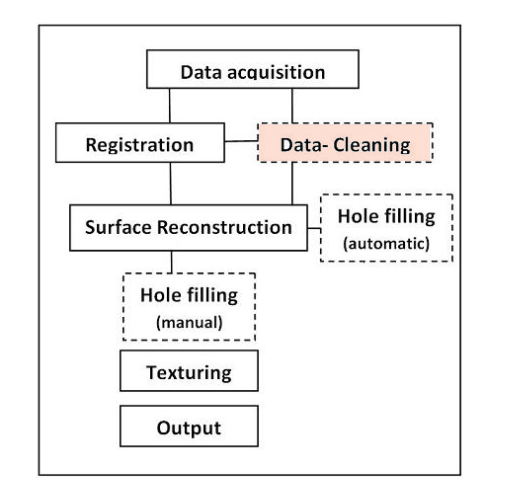
\includegraphics[width=0.45\textwidth]{pics/pipeline.png}
\caption{Processing pipeline \cite{Ruther2011}}
\label{fig:pipeline}
\end{figure}

% Scans have an intensity value, can have rgb
% Density of scans
% planar buildings
% there are no open source offerings
% land surveying, producing cad models, cultural heritage

The 3D models that is produced is the product of a processing pipeline that starts with data acquisition (see \autoref{fig:pipeline}) \cite{Ruther2011}. Laser rage scanners and cameras are used to capture the spatial domain. Following this, the point clouds acquired need to be cleaned and registered onto one coordinate space. Cleaning can be performed before or after registration. The surface reconstruction step triangulates the point cloud and produces a geometric model. Missing data or holes can be automatically filled during this step or manually afterwards. Finally, site photography is used to texture the model.

The focus of this project is on the cleaning step of this pipeline. Cleaning involves the removal of unwanted noise from point clouds. Noise can be classified into three categories. Static noise, dynamic noise and instrument noise. Static noise refers to unwanted objects that do not move. Examples can include vegetation, cars and equipment \cite{Held2012}. Dynamic noise are unwanted objects, such as birds or people, that move through the scan. Instrument noise occurs when part of laser beam hits a near object and part of it hits a far object. The result is that the average distance of the two objects is recorded.

A typical scan may take an experienced person anywhere between 30 minutes to 2 hours to clean. Given that one requires 500 - 1000 scans to cover a typical heritage site, this stage of the processing pipeline takes a considerable amount of time \cite{Ruther2011}.

In the Zamani project, vegetation is considered to be the most problematic type of noise \cite{Held2012}. The objective of this project is to develop a system to accelerate the removal of vegetation from point clouds.

In the next section shortcomings in existing systems and a overview of related work are presented. Subsequent sections will outline the project aims and research questions. Research methods will then be discussed. Finally the project time line will be presented.

\section{Background}

Point cloud cleaning implies the classification and segmentation of points corresponding to noise. This classification can be performed manually by the user or it can be automated. Various degrees of automation allow users to save time by offloading some aspects of a task to software. Automation can however compromise accuracy.

In the cultural heritage domain there is a strong emphasis on preserving detail. Every point is considered valuable information \cite{Held2012}. It is thus very important that noise is accurately classified.

\subsection{Existing systems}

\begin{table*}[htb]
\centering
  \begin{tabular}{| l | x{3cm} | x{3cm} | x{3cm} | c |}
  	\hline
	 & \multicolumn{3}{|c|}{Segmentation feature} & \\
	 \hline
	Package name & Simple & Semi automated & Fully automated & Open source \\    
    \hline
	Terrascan \cite{Terrasolid2012} & & & ground points, vegetation, buildings &	\tickNo \\
	\hline
	Pointools Edit \cite{Pointools2012} & lasso select\newline rectangle select, ball and cube brush select & floodfill with distance threshold, floodfill based on colour or intensity similarity, plane select & &	\tickNo \\
	\hline
	VR Mesh Studio \cite{VirtualGrid2012} & & power lines & ground, vegetation, roofs, planes &	\tickNo \\
	\hline
	Carlson PointCloud \cite{Carlson2012} & & & clear isolated and duplicate points, extract bare earth &	\tickNo \\
	\hline
	3D Reshaper \cite{Technodigit2012} & lasso select & & clustering with distance metric, clustering colours, remove isolated points &	\tickNo \\
	\hline
	Cyclone \cite{Leica2012} & lasso select & floodfill based on smoothness similarity &  &	\tickNo \\
	\hline	
	Meshlab \cite{VisualComputingLaboratory2012} & point picking & plane select & isolated point removal &	\tickYes \\
	\hline
  \end{tabular}
  \caption{Existing systems}
\end{table*}

Manual segmentation tools allow users to to achieve the highest degree of accuracy. Lasso selection is one such tool that is available in a number of commercial packages. \cite{Pointools2012,Leica2012,Technodigit2012}. It allows the user to draw a two dimensional polygon around points on screen. Unfortunately, hidden points behind the intended selection may be removed accidentally. For this reason it may be tedious to use when noise is hard to isolate. Despite it's shortcomings, lasso selection is currently the primary point cloud cleaning method used by members of the Zamani project \cite{Held2012}. Selection brushes lets the user select points by painting over them with a three dimensional brush. It can give a user more control over which points are removed \cite{Pointools2012} but is still time consuming.

A limited degree of automated cleaning can be achieved with different families of fill tools. Fill tools recursively add neighbouring points to a selection based on metrics such as distance or intensity \cite{Pointools2012}. Filling tools are however of little use because they fail to discriminate well between different types of objects. Pointools Edit \cite{Pointools2012} allows one to perform plane selection. While this tool is undoubtedly useful in many cases, not all selections are planar.

\begin{figure}[htb]
\centering
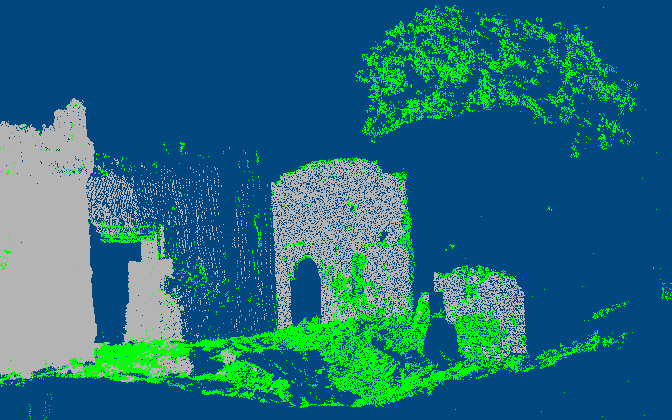
\includegraphics[width=0.45\textwidth]{pics/vrmesh-veg.png}
\caption{Automated segmentation of vegetation \cite{VirtualGrid2012}}
\label{fig:trees}
\end{figure}

Fully automated segmentation tools are found in many industrial packages. Packages exists that automatically segment a laser range scan into ground points, vegetation and buildings \cite{Terrasolid2012,VirtualGrid2012,Carlson2012}. Vegetation detection in VR Mesh Studio \cite{Terrasolid2012} is based on a noise metric. In the heritage domain buildings often exhibit uneven surfaces. Such surfaces can be mistaken for vegetation as is seen in \autoref{fig:trees}.

In 3DReshaper \cite{Technodigit2012} a point clustering approach is used to automatically segment a point cloud. Distinct objects are isolated by looking at the distance between neighbouring points. This approach may be somewhat effective on point clouds with a constant density. However, raw point clouds from laser scans decrease in density as one moves away from the origin. Applying this technique on a raw scan produces large clusters at the origin and increasingly smaller clusters as one moves further away (See \autoref{fig:dist}).

\begin{figure}[htb]
\centering
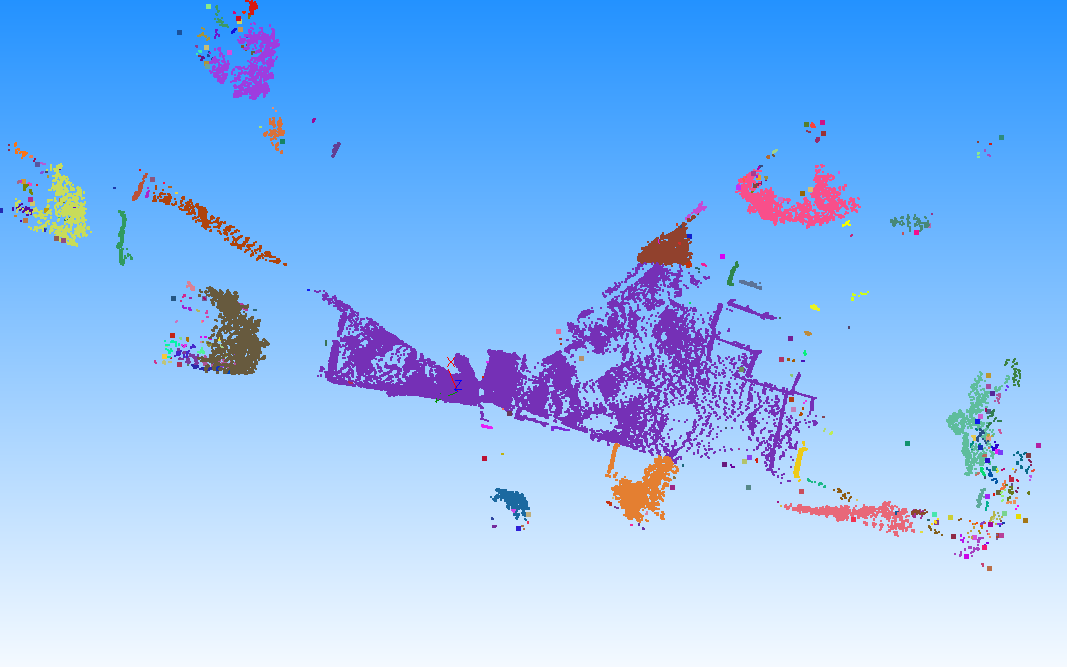
\includegraphics[width=0.45\textwidth]{pics/clustering.png}
\caption{Distance clustering \cite{Technodigit2012}}
\label{fig:dist}
\end{figure}

Meshlab \cite{VisualComputingLaboratory2012}, is the only known open source system that provides point cloud cleaning features. It is primarily aimed at processing triangulated meshes. Point cloud editing features were recently introduced in the form of point picking and plane selection tools. These features are somewhat slow when used on larger point clouds. They are also not sufficient to perform a point cloud cleaning task.

%For most industrial applications, once the necessary features in a point cloud have been identified, the level of detail is reduced by creating CAD models. The majority of point cloud editing packages cater for such applications. Segmentation tools from such packages may thus exhibit some inaccuracies that may lead to valid points being discarded which is unacceptable when working with heritage data.


%resolution of the scans are also different
% rotation table is higher
% land surveying is lower
% current workflow, select points into new layers using selection tools
% layers slow down

% no tools have been created specifically for this purpose
% cleaning can be done at various stages
% different cost benefits at different parts of the pipeline
% Meshlab, Meshedit

% system should take intensity values into account


\subsection{Related work}

% complex geopmetry cannot be discarded
% what is the model is simplified and then mapped to the complex points
% multi resolution kind of


Little research is available relating to the cleaning or classification of cultural heritage data. Extensive research has however been conducted in point cloud classification and segmentation in the context of robot navigation and other domains.

In robot navigation objects need to be identified in real time in order to inform actions. The general approach taken in such a classification task is to use point features to characterize basic surface characteristics. Subsequently machine learning techniques are used to classify points into higher level features. Point features can be far more efficiently calculated than alternative approaches such as model fitting.

Point features are calculated by considering the neighbourhood around a given point. A point normal is probably the most basic point feature. Fast Point Feature Histograms (FPFH) is a more complex point feature that has been shown to discriminate well between basic geometric surfaces \cite{Rusu2009}. \citeauthor{Rusu2009} used FPFHs to train both Conditional Random Fields (CRF) and Support Vector Machines (SVM) to classify basic geometric shapes. The classifiers where tested on a scan taken of a table scene with plates, cutlery and condiments. Different arrangements of the scene had between 70k and 80k points. Results showed that the CRF took 0.09 seconds to classify a point cloud with 97.36\% accuracy while SVM classified the cloud in 1.98 seconds with 89.67\% percent accuracy. FPFH in conjunction with CRFs for real time point cleaning of larger clouds seems promising. Cultural heritage data is however likely to exhibit far more noise. Using this unmodified approach to classify noise is not expected to produce acceptable results.

% only geometric features were used
A more complex approach was taken when attempting to recognize objects in urban environments. Urban datasets are more similar to the data that one is likely to find in the cultural heritage domain. \citeauthor{Golovinskiy2009} use a four step process to recognize objects. Firstly potential locations of objects are identified by looking at point density. Object are then isolated from background noise using graph cuts. To achieve this segmentation, two cost functions are introduced. The first penalizes neighbouring nodes being of a different type while the second cost function penalizes nodes that are far away from the object center. It was shown that this approach is superior to distance clustering. As in \cite{Rusu2009}, a classifier is trained and used to label isolated points. Unlike \cite{Rusu2009}, a feature vector describing the segmented shape is used. Shape features including spin images, shape volume and other features are used to classify objects such as cars and street lights. Contextual features such as the distance of an object from a known feature such as a road are also taken into account. After features have calculated the final step is classification. Random forest, k-nearest neighbours and SVM were tested. SVM was most accurate and correctly classified 65\% of objects.

%This approach my not be cleaning. But the ideas cloud be applied to point cloud cleaning. Specifically graph cuts and taking contextual information into account

Automatic segmentation of cultural heritage sites into surfaces and edges was demonstrated by \citep{Spina2010}. What makes the segmentation of heritage data hard, is that scanned structures can exhibit very complex geometries that are hard to classify \cite{Spina2010}. The point feature used was the ratio of the two largest eigenvalues after a Principle Component Analysis of a point's neighbourhood. It was shown to be effective in segmenting sites into planes and edges.

A variety of point feature schemes that are used extensively in robotics, could potentially be exploited in the cultural heritage domain. A number of popular point feature algorithms have been implemented and are freely available in the Point Cloud Library \cite{Rusu2011}.

% Talk about wang

%seperate trees for sites

%Segmentation algorithms generally have two passes. The first pass sees that individual points are classified. In the second pass, segmentation is performed by grouping point features into groups that correspond to objects or parts thereof.

% What is the difference between point classification and point segmentation

%Segmentation means to divide up the image into a 
%patchwork of regions, each of which is “homogeneous”, 
%that is, the “same” in some sense
%– Intensity, texture, colour, …
%• Classification means to assign to each point in the image 
%a tissue class, where the classes are agreed in advance
%– Grey matter (GM), White matter (WM), cerebrospinal fluid (CSF), 
%air, … in the case of the brain

%\subsection{Artifacts types}

\section{Aims}
From the above review of point cloud classification and segmentation literature it seems unlikely that automated cleaning of laser scans could achieve the accuracy required by the cultural heritage community. It is therefore proposed that an augmented approach be taken to enhance a persons ability to isolate local noise in a fast and accurate manner. In order to limit the scope of this project while maximising impact, the focus of this project will be on the removal of vegetation. This will include trees, shrubs and grass.

%The aim of this research is to produce a system that will allow users to clean cultural heritage data in a fast and effective manner. The focus will be on finding ways to remove the most problematic artefacts as identified by the Zamani project. In descending order of importance, the focus will thus be on removing vegetation, people, and equipment. 

%Existing point feature schemes will be investigated, as well as heuristic and machine learning approaches to segmentation. In order to ensure fast response times, cleaning methods will be accelerated with OpenCL.

\section{Research question}

TODO: Explain more
\begin{itemize}
\item To what extent can augmented methods speed up the segmentation of vegetation?
\item What degree of accuracy can be obtained?
\end{itemize}

\section{Method}
The proposed method of vegetation removal will let the user limit the search space by isolating the approximate area containing the target vegetation. A lasso tool will be implemented for this purpose. In the case of a bush or a tree, the user will be asked to select the center of the object using a point picking tool. 

Given the search space and a point lying on the object, heuristic together with contextual cues will be used to segment a tree. Contextual cues such as the location of the ground plane could be used in order to inform a heuristic algorithm. A tree generally has a cylindrical trunk and a leafy crown higher up. A heuristic algorithm can be created to expect point features to become more noisy further up away from the ground as the crown of the tree is approached. Such heuristics can be encoded as an energy function and be used with a graph cut algorithm in order to segment vegetation. \footnote{Given that scans overlap to some extent in order to perform registration, an extension could be written to apply cleaning from a cleaned scan to a dirty overlapping scan. PCL contains a registration module which could be used for this purpose.}

An alternative approach to investigate is the use of trained classifiers such as SVM's or CRF's to classify points that are likely to correspond to a vegetation.


% registration based cleaning
\section{System}

The development of the segmentation method with proceed incrementally. The first step will be to create a user interface in which segmentation methods can be tested. The goal will then be to segment free standing trees, shrubs and grass. Once this has been completed trees and shrubs that co-occur with buildings will be segmented. Once serial methods have been implemented an attempt will be made to improve performance using GPGPU techniques. The calculation of most point features generally only involves local data dependencies is thus an ideal candidate for a GPGPU implementation. Graph cuts have also been shown to be parallelisable on GPUs \cite{Hussein2007}.

The system will be designed to process single scans in Leica PTX format, as this is what the Zamani Project uses \cite{Held2012}. Existing point features in the PCL library \cite{Rusu2011} will be used. The interface will use QT and OpenGL, while OpenCL will be used for GPGPU algorithms.

\section{Evaluation}

The system will be evaluated both quantitatively and qualitatively. In the quantitative evaluation it will be determined whether the new system outperforms the old system in terms of speed and accuracy. For the qualitative evaluation an expert opinion will be acquired.

For the quantitative evaluation members of the Zamani group will be recruited as well as their interns. A counterbalanced repeated measures design will be used due to the limited number of experienced users that will be available for testing. Users will be given a number of scans to clean. The scans will have to be cleaned using both Leica Cyclone and the new system. To counteract practise effects the order in which the two systems will be used will vary between users. In order in which scans will be cleaned will also be shuffled. The cleaning task will be timed and accuracy will be determined by comparing user cleaned scans with pre-cleaned scans. A basic point cloud diff tool with be created for this purpose.

% how big of a sample?
% what about significance

The system will qualitatively be evaluated by walking an experienced member of the Zamani project through the cleaning process while conducting an interview.
			
%What about pairwise registration and scanning framework?

\section{Milestones}
\begin{table}[h]
\begin{tabular}{llr}
\hline
Task & Due date \\
\hline
Research Proposal & June 2012\\
Point Cloud Cleaning Framework & July 2012\\
Basic Cleaning Tools & August 2012\\
Clean Isolated Vegetation & September 2012\\
Background Chapter & November 2012\\
Clean All Vegetation & January 2013\\
System Design Chapter & February 2013\\
Implementation Chapter & March 2013\\
User testing & April 2012\\
Evaluation Chapter & May 2013\\
Thesis Draft & June 2013\\
Conference Paper & July 2013\\
Final Draft & August 2013\\
\hline
\end{tabular}
\end{table}

TODO: Gantt chart

%by comparing the time taken to clean a scan with Zamani's current system \cite{Leica2012} to the new system.

% compare on a feature to fearure basis and wholesale?

% user centered design???

% user study:
% how fast clean cloud before
% for fast clean cloud after
% qualitative overview

%cleaning should be done in real time
%user testing
%focus on the problems that will have the biggest effect in terms of time savings

% Should allow them to edit accurately on a specific subspace

%\section{Methods}
%Find and classify the problems that are most difficult and time consuming

%Chris:
%    Biggest problems are:
%		Vegetation (Hard to select trees)
%		People walking through scans
%		Boxes such as equipment lying around
%
%	Problem is that useful features are scattered across many systems
%	Systems are proprietary
%	
%Systems:
%	Cyclone:
%		Select surfaces based on smoothness metric (Fuckin slow)
%		Use lasso tool
%	Pointools
%		Brush select
%	Kubit
%	Alice labs studio clouds
%	Meshlab (really hard to select things)
%	XGRT: Deals with very large clouds
%		
%		
%Desires:
%	Intelligent select
%		Eg. select table and only select surface
%	Brush type tool (Pointools):
%		Selects points based on intensity values
%	
%	Selection tools for a variety of objects
%		How to do?
%		Enumerate all types?
%		Or create some type of dynamic learning system

\bibliographystyle{plainnat}
\bibliography{proposal}	

\end{document}
